
\section{Local Filtering and Edge Detection}

\subsection{Filtering}
The naive approach to local filtering involves taking a simple moving average of the pixels in the neighborhood.

\subsection{Convolution}
Convolution entails convolving an input matrix (the input image) with a \textbf{kernel},
a matrix defining weights for each element in the neighborhood.
This operation can be seen as a moving weighted average of pixels.
\begin{center}
    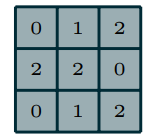
\includegraphics[width=0.4\linewidth]{img/Kernel_Convolution}
\end{center}
The kernel slides across the input matrix, computing the product between each kernel element and the corresponding input element.
The results are summed to obtain the output at the current location.
If the input matrix has $i$ rows and the kernel has $k$ rows, the output will have $i-k+1$ rows (and columns).

\begin{center}
    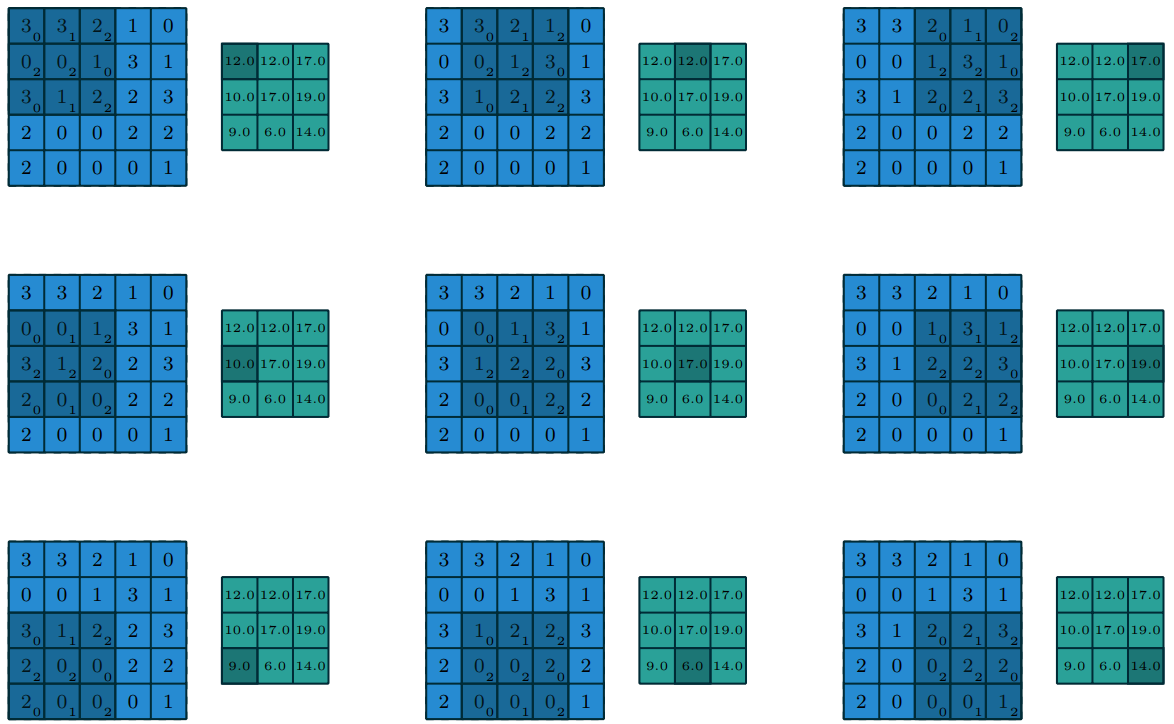
\includegraphics[width=0.8\linewidth]{img/ConvolutionOutput}
\end{center}

\subsection{Edge Detection}
Edge detection, challenging in image processing, identifies edges based on rapid intensity changes,
which can be captured by calculating the derivative.

\begin{center}
    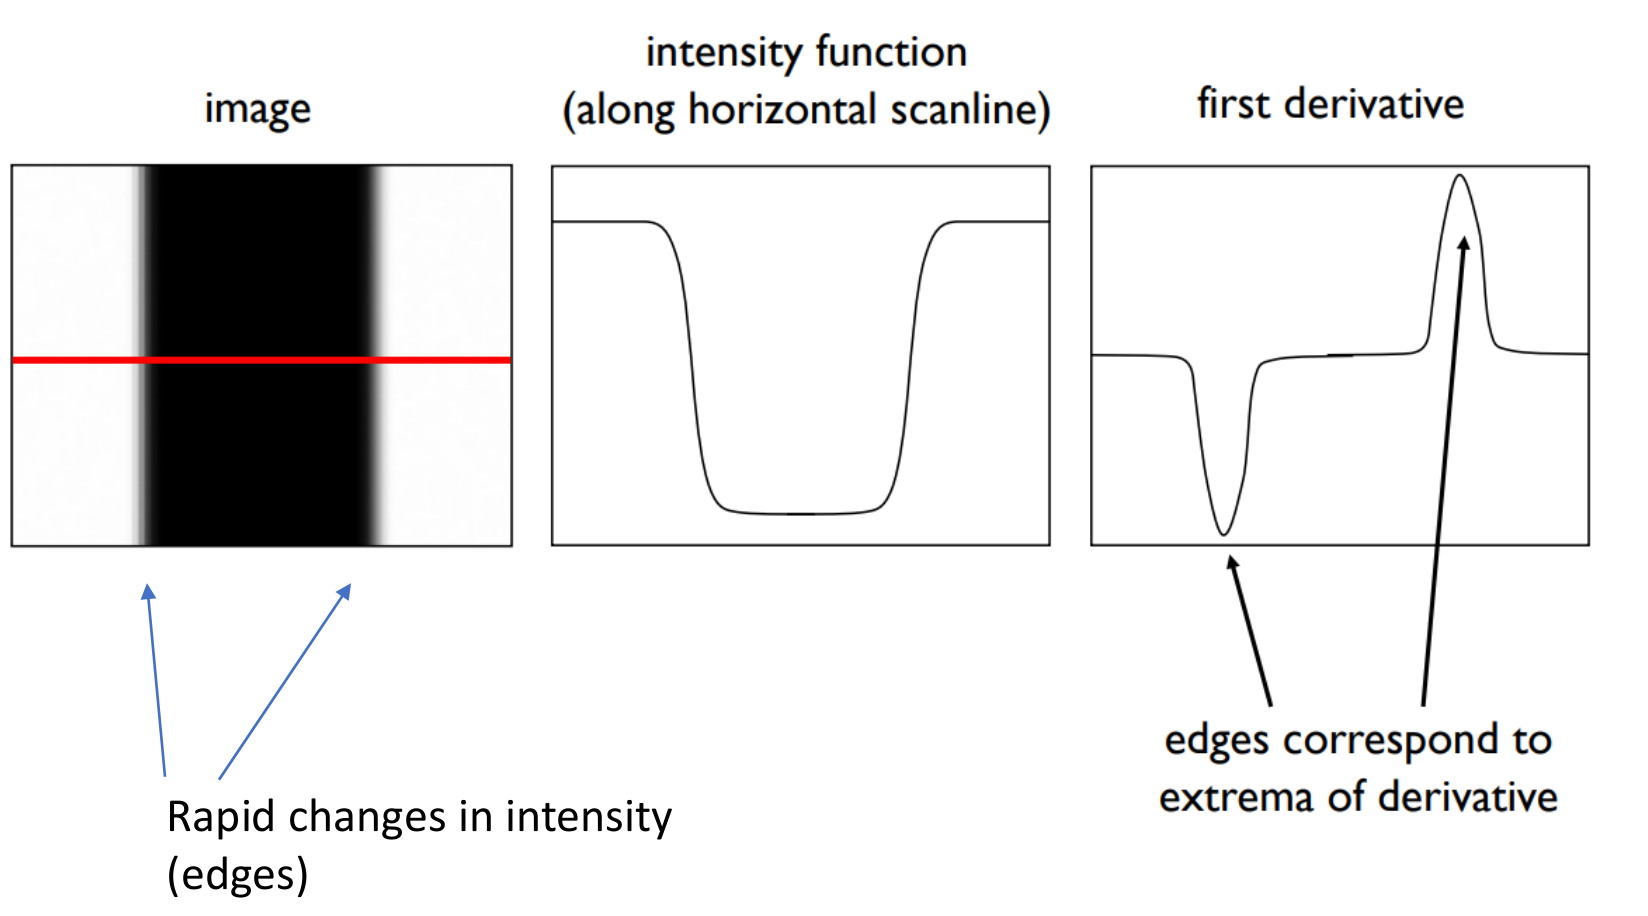
\includegraphics[width=0.6\linewidth]{img/1D_edge_derivative}
\end{center}

In two dimensions, the derivative corresponds to the gradient $\nabla f = \left[\frac{\partial f}{\partial x},\frac{\partial f}{\partial y}\right]$,
pointing from the edge towards the intensity increase or the lighter side.

\begin{align}
    & \text{Gradient} & \nabla f &= \left[ \frac{\partial f}{\partial x}, \frac{\partial f}{\partial y} \right] \\
    & \text{Gradient Direction} & \theta &= \tan^{-1} \left( \frac{\partial f}{\partial x} / \frac{\partial f}{\partial y} \right) \\
    & \text{Gradient Magnitude (or Modulus)} & \norm{\nabla f} &= \sqrt{\left(\frac{\partial f}{\partial x}\right)^2 + \left(\frac{\partial f}{\partial y} \right)^2 }
\end{align}

However, not all significant edges have strong gradients, nor are all strong gradients indicative of important edges.

\subsubsection{Computing the Gradient on an Image}
The approximate gradient in the $ \frac{\partial f}{\partial x} $ direction is obtained by convolution with the kernel \begin{tabular}{|c|c|}
    \hline
    -1 & 1\\
    \hline
\end{tabular}

The approximate gradient in the $ \frac{\partial f}{\partial y} $ direction is obtained by convolution with the kernel \begin{tabular}{|c|}
    \hline
    -1 \\
    \hline
    1\\
    \hline
\end{tabular}

The drawback of the gradient is its sensitivity to noise, which can be addressed by first smoothing the function and then applying the gradient.

\begin{figure}[H]
    \centering
    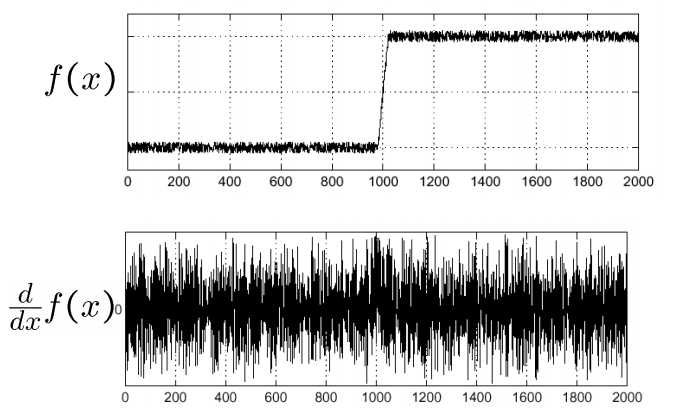
\includegraphics[width=0.7\linewidth]{noise_gradient}
    \caption{Gradient of a 1D function, illustrating noise amplification and potential signal concealment.}
    \label{fig:noisegradient}
\end{figure}

The solution is to smooth the function first, and then apply the gradient.
A convolution with a derivative of the Gaussian filter is often used for this purpose,
equivalent to smoothing with a Gaussian and then taking the derivative.

\begin{figure}[H]
    \centering
    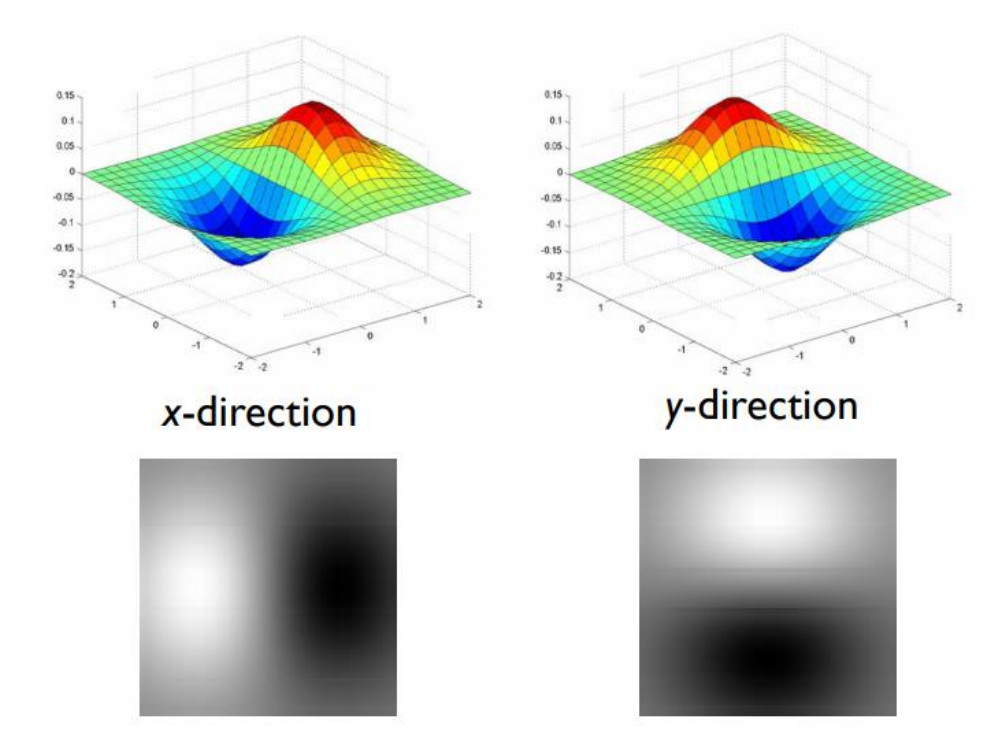
\includegraphics[width=0.6\linewidth]{img/derivative_gaussian_filter2}
    \caption{Derivative of Gaussian Filters. A Gaussian smoothing filter removes high-frequency components,
	and derivative filters yield large responses at points with high contrast.}
    \label{fig:derivativegaussianfilter2}
\end{figure}

\subsection{Canny Edge Detection}
Canny Edge Detection follows a similar approach but includes edge thinning and hysteresis thresholding for enhanced performance.
The steps include:
\begin{enumerate}
    \item Approximating gradients along axes using derivative of Gaussian filters.
    \item Computing gradient magnitude.
    \item Making edges one pixel wide through non-maxima suppression along the perpendicular direction to the edge.
    \item Keeping only strong edges through hysteresis thresholding.
\end{enumerate}

\subsection{Hysteresis Thresholding}

\begin{wrapfigure}{R}{0.4\textwidth}
    \centering
    \vspace{-16mm}
    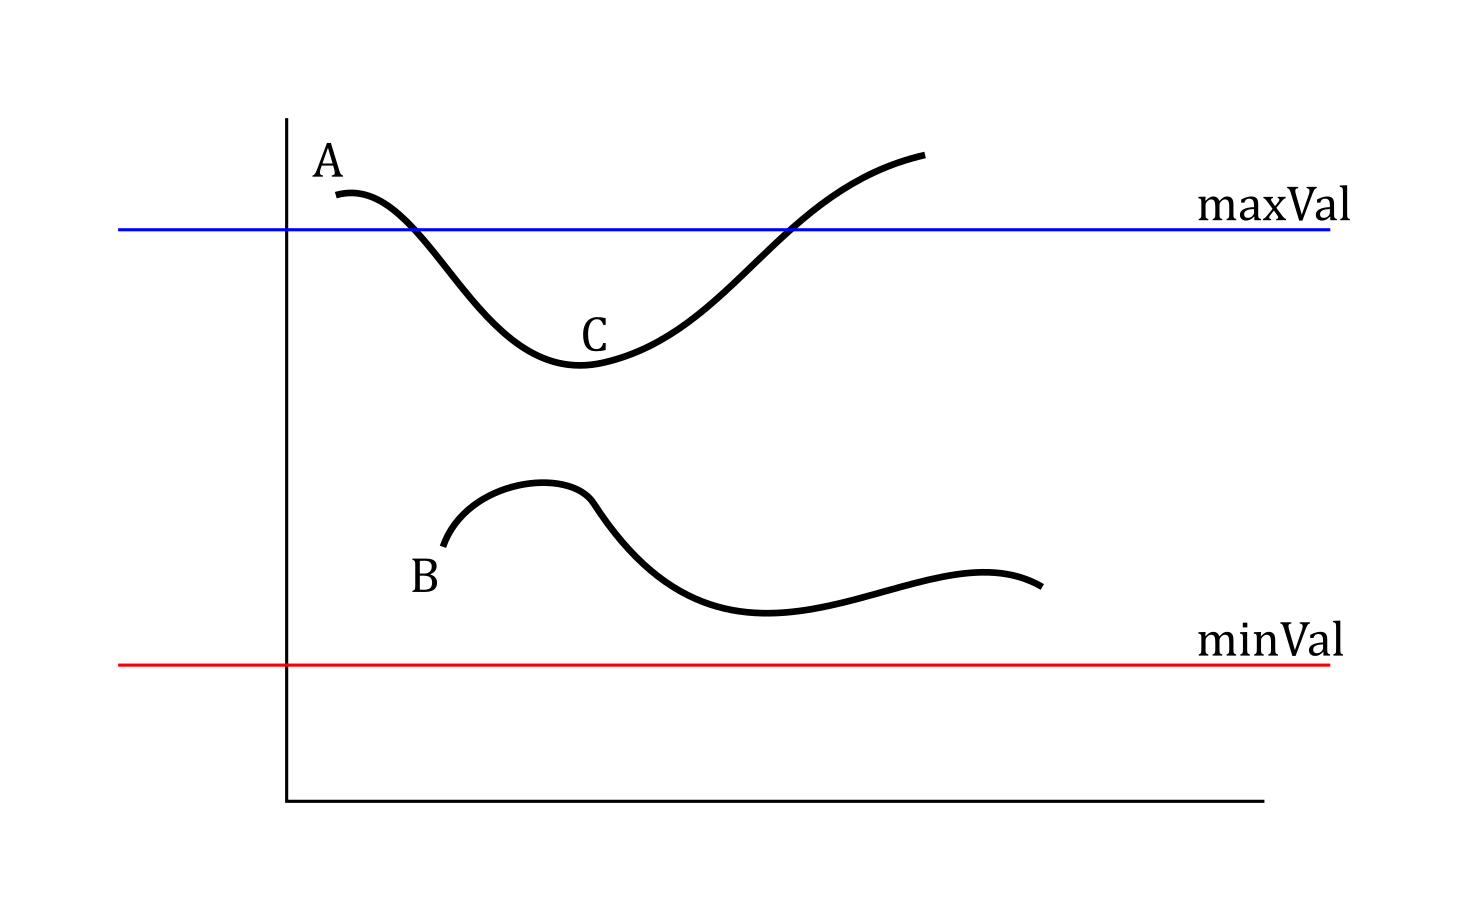
\includegraphics[width=\linewidth]{hysteresis_thresholding}
    \vspace{-20mm}
\end{wrapfigure}

This stage determines genuine edges by employing two threshold values, \texttt{minVal} and \texttt{maxVal}.
Edges with an intensity gradient surpassing \texttt{maxVal} (A) are definitively identified as edges,
while those falling below \texttt{minVal} are discarded as non-edges.
Pixels lying between these thresholds are classified based on connectivity: if connected to "sure-edge" pixels (C),
they are deemed part of edges; otherwise (B), they are also discarded.
